% 1977 年广西卷（理科）第 4 题：正四棱锥 V-ABCD，O 为底面正方形中心（高的垂足），
% 实线：可见侧棱 VA、VB、VC 与底边 AB、BC；虚线：侧棱 VD、底边 AD、DC、高 VO、底面对角线半段 AO、DO（按源卷第 3 页布局）
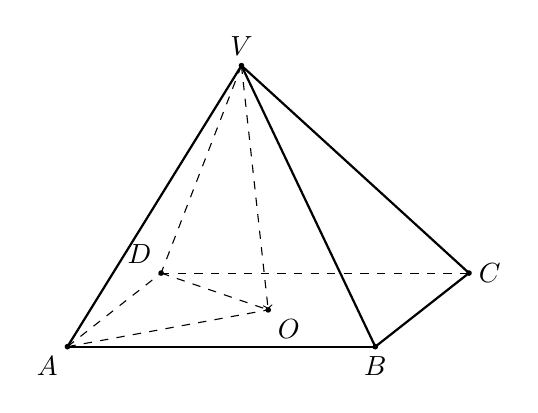
\begin{tikzpicture}[scale=0.85]
  \coordinate (A) at (0,0);
  \coordinate (B) at (4.6,0);
  \coordinate (C) at (6,1.1);
  \coordinate (D) at (1.4,1.1);
  \coordinate (O) at (3,0.55);
  \coordinate (V) at (2.6,4.2);
  \draw[thick] (V)--(A);
  \draw[thick] (V)--(B);
  \draw[thick] (V)--(C);
  \draw[thick] (A)--(B);
  \draw[thick] (B)--(C);
  \draw[dashed] (V)--(D);
  \draw[dashed] (A)--(D);
  \draw[dashed] (D)--(C);
  \draw[dashed,->] (V)--(O);
  \draw[dashed] (A)--(O);
  \draw[dashed] (D)--(O);
  \fill (A) circle (1.2pt) node[below left] {$A$};
  \fill (B) circle (1.2pt) node[below] {$B$};
  \fill (C) circle (1.2pt) node[right] {$C$};
  \fill (D) circle (1.2pt) node[above left] {$D$};
  \fill (O) circle (1.2pt) node[below right] {$O$};
  \fill (V) circle (1.2pt) node[above] {$V$};
\end{tikzpicture}
